% Chapter 4

\chapter{Extracción de características del iris en condiciones no ideales} % Main chapter title

\label{Capítulo 4} % For referencing the chapter elsewhere, use \ref{Chapter4} 

%----------------------------------------------------------------------------------------

% Define some commands to keep the formatting separated from the content 
%\newcommand{\keyword}[1]{\textbf{#1}}
%\newcommand{\tabhead}[1]{\textbf{#1}}
%\newcommand{\code}[1]{\texttt{#1}}
%\newcommand{\file}[1]{\texttt{\bfseries#1}}
%\newcommand{\option}[1]{\texttt{\itshape#1}}

%----------------------------------------------------------------------------------------

\section{Introducción}





%----------------------------------------------------------------------------------------

\section{Descripción del método propuesto}



\begin{figure}[htbp]
\centering
\subfigure[S1001L06.jpg]{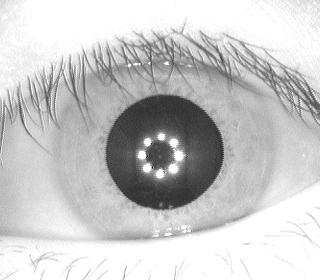
\includegraphics[width=44mm]{tfm-img16}}
\subfigure[S1113R05.jpg]{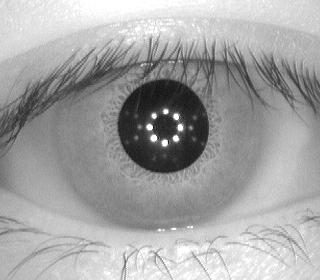
\includegraphics[width=44mm]{tfm-img17}}
\subfigure[S1188L04.jpg]{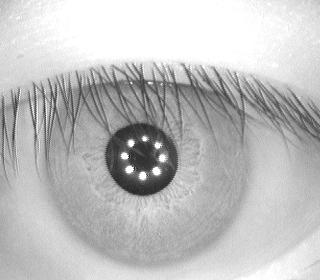
\includegraphics[width=44mm]{tfm-img18}}
\subfigure[S1200R02.jpg]{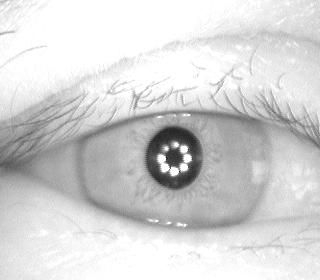
\includegraphics[width=44mm]{tfm-img19}}
\subfigure[S1217L04.jpg]{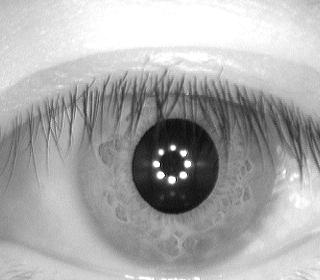
\includegraphics[width=44mm]{tfm-img20}}
\caption{Imágenes de la base de datos CASIA-IrisV4.} \label{fig:señales}
\end{figure}

%----------------------------------------------------------------------------------------